\documentclass[12pt]{article}
\usepackage{sbc-template}
\usepackage{graphicx,url}
\usepackage[utf8]{inputenc}
\usepackage[brazil]{babel}
%\usepackage[latin1]{inputenc}  
\usepackage{comment}
\usepackage{color}
\usepackage{xcolor}
\newcommand{\cristina}[1]{\textcolor{red}{#1}}

\sloppy

\title{Avaliação de Métodos de Roteamento de Fonte para Engenharia de Tráfego em Aplicações de\\ Ciência de Dados Intensiva}

\author{Domingos J. P. Paraiso\inst{1}  }

\address{Programa de Pós-graduação em Computação Aplicada (PPComp)\\
Campus Serra do Instituto Federal do Espírito Santo (IFES)
\email{domingos.paraiso@gmail.com}
}

\begin{document} 

\maketitle

\begin{abstract}
  This paper presents the requirements of Data Intensive Science applications and proposes source routing protocols as a way to comply with these requirements. The Segment Routing protocols present in some commercial switches and PolKA, which presents a deterministic way of defining the route, were explored. The focus of the tests were full use of 100 Gbps links using flow aggregation, used in scientific research networks, change of service instance through tunnel migration, load balancing and fault tolerance.
\end{abstract}

\begin{resumo} 
  Este artigo apresenta os requisitos das aplicações de Ciência de Dados Intensiva e propõe que sejam utilizados protocolos de roteamento na origem como forma de cumprir com estes requisitos. Foram explorados os protocolos Segment Routing presente em alguns \textit{switches} comerciais e o PolKA que apresenta uma forma determinística de definição de rota. O foco dos testes realizados foram agregação de fluxo para utilização completa de enlaces de 100 Gbps, usados nas redes de pesquisas científicas, mudança de instância de serviço por meio de migração de túnel, balanceamento de carga e tolerância à falhas.
\end{resumo}

\section{Introdução}

%Motivação, contexto e estado da arte

Pesquisas científicas atuais têm gerado conjuntos de dados digitais na escala de petabytes por meio de detectores, simulações e análises \cite{zurawski2021}. Muitas destas pesquisas exigem colaboração com outras instituições e pesquisadores geograficamente dispersos pelo mundo \cite{babik2020network}. A troca de informações entre os envolvidos exige que grande parte desse enorme volume de dados seja compartilhado para consumo, análise e apresentação de resultados em tempo hábil para dar suporte a aplicações de Ciência de Dados Intensiva (do inglês \textit{Data Intensive Science}) \cite{guiang2022integrating}.

Várias redes de alto desempenho de pesquisa e educação estão interconectadas e tem implantado sistemas de reserva de circuitos entre domínios, como a Energy Sciences Network (ESnet) nos Estados Unidos, que apoia os experimentos do LHC (do inglês \textit{Large Hadron Collider}) \cite{8665783}, e a GÉANT \cite{valera2019geant} que interliga vários centros de pesquisa na Europa.
%
Os centros de pesquisa estão cada vez mais conectados por redes de alto desempenho, atualmente são usados enlaces de 100Gbps mas é esperado que se chegue a taxa de Terabytes nos próximos anos  \cite{zurawski2021}. É importante que sejam escolhidos meios que suportem os requisitos de comunicação das aplicações usadas nas pesquisas. 

Para otimizar a eficiência das redes, devem ser escolhidas ferramentas e métodos que permitam um uso mais racional dos recursos disponíveis a fim de conseguir um aumento na eficiência geral da rede, levando ao atendimento dos níveis de QoS (Qualidade de Serviço, do inglês \textit{Quality of Service}) dos projetos. Alguns dos recursos que vão colaborar para que as redes suportem os requisitos são: possuir algum tipo de tolerância à falhas e uma administração centralizada, ágil e simplificada.
Além disso, as aplicações de ciência de dados intensivas exigem a troca de grandes volumes de dados entre centros de pesquisa no menor tempo possível, para que isso seja feito de forma eficiente a largura de banda do enlace entre as instituições deve ser o mais próximo da sua capacidade total utilizando todas as rotas disponíveis.

%Problema e Hipótese

Uma possível solução para atendimento a esses requisitos é o uso da TE (Engenharia de Tráfego, do inglês \textit{Traffic Enginering}) na rede. Entretanto, os mecanismos de TE dos protocolos tradicionais de roteamento não permitem atualizar dinamicamente os melhores caminhos para utilizar a capacidade total da rede de forma mais eficiente. Esse problema é intensificado devido aos requisitos mais rigorosos no tráfego devido ao grande volume de dados, no contexto de Ciência de Dados Intensiva \cite{babik2020network}.

Para preencher essa lacuna, uma alternativa promissora é o uso de protocolos do tipo \textit{Source Routing}, que fazem a troca dinâmica de rotas de forma mais ágil que as técnicas tradicionais, porque só necessitam atualizar as regras nos nós de entrada, já que um rótulo de rota será inserido no cabeçalho dos pacotes e os nós internos só precisam fazer operações neste rótulo. Esses protocolos podem ser classificados como: (1) \textit{Loose Source Routing}, quando eles indicam alguns pontos da rede por onde o pacote deve passar e, nos casos onde o caminho não é explícito, os roteadores utilizam os métodos tradicionais; e (2) \textit{Strict Source Routing}, que definem objetivamente todos os saltos entre a origem e o destino, permitindo um detalhamento completo da rota. 

Apesar de existirem muitos estudos nesta área como \cite{schuller2018traffic} que faz a análise do fluxo em um grande provedor de acesso e \cite{kushwaha2020survey} que explora o uso do protocolo em diversos cenários. Nenhum deles são aplicados diretamente ao problema de transferência de altos volumes de dados e fluxos agregados.
 
O \textit{Segment Routing} (SR) \cite{abdullah2018segment}, que é do tipo \textit{Loose Source Routing}, é o protocolo de \textit{Source Routing} mais adotado e disponível em equipamentos comerciais. Existem diversos trabalhos que investigam funcionalidades de TE usadas no SR, mas não foi encontrada na literatura uma avaliação do protocolo que leve em conta os requisitos de Ciência de Dados Intensiva. 
Também não foram encontrados trabalhos na literatura que comparem o SR com outros protocolos de \textit{Source Routing}, apenas entre a proposta original do SR e algumas propostas de melhoria. 
Assim, é importante fazer uma comparação entre o SR e algum outro protocolo do tipo \textit{Strict Source Routing}, de forma a avaliar se os protocolos de \textit{Source Routing} existentes cumprem com os requisitos demandados pelas aplicações de Ciência de Dados Intensiva.

Existem ainda algumas limitações para o uso do SR, como o \textit{Maximum SID Depth} (MSD), que é o limite de saltos informados na origem e varia de acordo com a capacidade do equipamento. Além disso, existe uma sobrecarga gerado na modificação dos pacotes causada pela retirada de rótulos dos segmentos por onde o pacote passou. É necessário entender quais são as alternativas na literatura que contornam este problema e avaliar essas opções em relação aos requisitos de TE. 

Com essa motivação, esse trabalho propõe a comparação entre os protocolos \textit{Segment Routing} e o PolKA \cite{dominicini2020polka}, que é do tipo \textit{Strict Source Routing}, identificando se eles conseguem atender aos requisitos de rede das aplicações de ciência de dados intensiva.

Como contribuição este artigo apresenta os requisitos das redes para aplicações de Ciência de Dados Intensiva e como estes requisitos podem ser atendidos quando são usados protocolos de roteamento na origem por meio da comparação dos seus comportamentos em \textit{testbeds} locais emulados e em \textit{testbeds} físicos remotos.

Os dois protocolos testados apresentaram resultados similares e são alternativas interessantes para uso nas redes científicas que necessitam de alta vazão, agilidade na mudança de rotas, tolerância à falhas e balanceamento de carga.

O \textit{Segment Routing} por estar presente na instalação de fábrica em \textit{switches} comerciais possui mais opções disponíveis para uso imediato, em alguns equipamentos mais antigos o número de segmentos pode estar limitado devido à implementação do tamanho da pilha MPLS. O PolKA necessita que os equipamentos possuam suporte à linguagem P4 e acesso ao módulo de cálculo de CRC que permita a configuração do polinômio a ser usado, mas tem a vantagem de explicitar cada salto da rota escolhida.

%Estrutura do artigo

Este artigo está estruturado da seguinte forma, na Seção 2 comparamos com os trabalhos relacionados, a Seção 3 apresenta a estruturação dos testes, a seção 4 os resultados obtidos e na Seção 5 a conclusão e trabalhos futuros.

\section{Trabalhos relacionados}

Existem trabalhos que fizeram análises de redes para aplicações de Ciências de Dados Intensiva, trabalhos que analisaram o protocolo \textit{Segment Routing} e trabalhos com a proposta do protocolo PolKA.

O paper \cite{ioannou2020data} nos mostra que projetos de pesquisas em física de alta energia, genoma e astronomia geram um grande volume de dados que muitas vezes precisam ser transferidos para outros locais. Este mesmo documento cita que tem sido usadas ferramentas para criar uma DMZ de redes científicas onde são instalados os \textit{Data Transfer Nodes} (DTNs), que são conjuntos de hardware e software com grande velocidade de leitura e gravação além de ferramentas de transferência de dados que precisam atingir taxas de, pelo menos, 100Gbps. Também cita que as redes \textit{European National Research and Education Networks} (NRENs) possuem enlaces de alta capacidade, e que o GÉANT é a colaboração das NRENs, possuindo um serviço de \textit{testbeds} que segue os princípios de boas práticas da DMZ científica. Os requisitos são: uma rede de alta capacidade com políticas específicas para os fluxos de trabalho das pesquisas, DTNs de alta performance e instrumento de medida de performance da rede. Uma política de uso das redes separa o tráfego local do campus que continua passando pelo \textit{firewall} enquanto a DMZ é tratada de forma mais eficiente, sem uma inspeção mais profunda do conteúdo dos pacotes. Além disso, descreve como o \textit{tunning} do Kernel do Linux melhorou a performance de rede. Apesar disso, em todos os testes a velocidade máxima não atingiu 10Gbps em função do conjunto de hardware e software utilizados.

O paper \cite{elaineyeo2019} apresenta o \textit{Segment Routing} como uma solução para simplificar e otimizar uma rede atingindo os requisitos de latência e eficiência operacional em um grande provedor de acesso. O resultado oferece a indicação de mudar a arquitetura ou continuar com o RSVP-TE (do inglês \textit{Resource Reservation Protocol for traffic engineering}). O estudo informa que, apesar do protocolo usado ter a habilidade de refazer as rotas com rapidez, ele é complicado para escalar pois os equipamentos no core da rede precisam ficar mantendo o estado das rotas. Dessa forma o uso do \textit{Segment Routing} foi testado com resultado positivo, pois proporciona a inclusão da rota de cada pacote apenas pelos nós de entrada, além de permitir uma visão geral da rede de forma centralizada.

Como resultado do teste, que avaliou o uso do \textit{Segment Routing} sobre o MPLS, foi identificado que o Maximum SID Depth (MSD), indicador do número máximo de segmentos que poderão ser especificados no pacote, está limitado ao tamanho máximo de \textit{labels} MPLS suportado pelos dispositivos usados no teste, este número ficou entre 3 e 16. O estudo concluiu que, apesar do alto custo de equipamentos que suportem o \textit{Segment Routing}, existe um retorno de investimento na diminuição da complexidade de manter a rede e redução das multas por não atingir os níveis de SLA, além de ter uma rede escalável e com uma visão geral centralizada. Como ponto negativo, fica a conclusão de que as implementações dos fabricantes não possuem os mesmos recursos implementados gerando dificuldade na sua interoperabilidade. O estudo não fez comparação com outras alternativas.

O survey de \cite{kushwaha2020survey} apresenta a aplicação do \textit{Segment Routing} em vários planos de dados, diversos esquemas de \textit{Label Encoding} e sua implementação em \textit{switches} comerciais, apesar de não fazer comparações com outros protocolos. Além disso, faz um resumo sobre as possibilidades de aplicação do SR em redes de provedores de acesso, grandes empresas e \textit{datacenters}. Discute sobre o uso em campus mas apenas para indicar o uso do protocolo na segmentação do tráfego, possibilitando melhorar a qualidade de usuários específicos.

O trabalho de \cite{schuller2018traffic} analisa dados históricos de provedores de acesso na europa com informações sobre o tráfego local e intercontinental e realiza alguns estudos sobre os horários de pico e as melhorias que poderiam ser obtidas com o uso do protocolo \textit{Segment Routing}. Por fim, o trabalho faz uma análise de tráfego real comparando o \textit{Segment Routing} com protocolos tradicionais e com modificações feitas por extensões aplicadas ao \textit{Segment Routing}. Apesar de não o comparar com outros protocolos de \textit{Source Routing}, este estudo explorou como as extensões se comportam variando alguns de seus parâmetros face às outras opções.

O foco principal da pesquisa de \cite{dominicini2021deploying} é apresentar como implementar o protocolo PolKA em um \textit{switch} com suporte à linguagem P4 no plano de dados, além da implementação é feita uma comparação com um protocolo de \textit{Port Switching} implementado na mesma arquitetura. Além da implementação em um protótipo simulado, também foi feita em hardware usando \textit{switches} Tofino da Intel e foram realizados alguns testes de \textit{Throughput} e \textit{Forwarding latency}. Como resultado, os testes indicaram que o PolKA ofereceu performance equivalente ao \textit{Port Switching} indicando ser uma alternativa viável para ambientes onde um protocolo do tipo \textit{Strict Source Routing} seja relevante mas não foi explorado o uso completo dos enlaces disponíveis nem comparado a outro protocolo do tipo \textit{Source Routing}.

A pesquisa busca comparar dois protocolos de \textit{Source Routing} de tipos diferentes, o \textit{Segment Routing} do tipo \textit{Loose Source Roting} e o PolKA do tipo \textit{Strict Source Routing} avaliando se eles conseguem atender aos requisitos das aplicações de Ciência de Dados Intensiva. Isso foi feito avaliando a utilização completa de enlaces de 100Gbps usando fluxos agregados, migração dinâmica de rotas e suporte ao recurso de tolerância à falhas.

\begin{table}[ht]
\centering
\caption{Comparação entre as análises realizadas pelos artigos correlatos}
\label{tab:Tabela1}
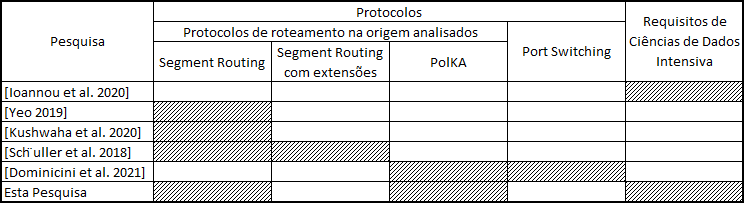
\includegraphics[width=.7\textwidth]{tabela1.png}
\end{table}

\section{Proposta do Artigo}

A proposta deste artigo é testar a que nível os protocolos \textit{Segment Routing} e PolKA conseguem atender aos requisitos das Aplicações de Ciência de Dados Intensiva. Serão realizados testes em dois \textit{testbeds} um local e outro remoto. Como diferenciais sobre os outros trabalhos relacionados, temos a comparação de dois tipos de protocolos de \textit{Source Routing} e suas implicações quando submetidos a cargas de dados buscando obter o máximo rendimento dos recursos de rede disponíveis.

O \textit{Segment Routing} é um protocolo do tipo \textit{Source Routing} que é padronizado pelo IETF, sua arquitetura é mantida pelo grupo \textit{Source Packet Routing in Networking} (spring) \cite{gang2018throughput}. Ele inclui no nó de entrada uma lista de segmentos, que são instruções a serem seguidas pelos nós no caminho, essa lista pode ser implementada como \textit{labels} MPLS ou dentro do IPv6. Segmentos podem indicar um nó específico ou um segmento de rede, dentro desse segmento o roteamento é feito usando os protocolos tradicionais até atingir o nó que vai encaminhar ao próximo segmento. Os experimentos realizados utilizam a implementação do \textit{Segment Routing} que usa labels MPLS, ficando fora dessa avaliação a implementação em IPv6 pois a maioria das implementações em equipamentos de produção só suporta MPLS. O \textit{Segment Routing} é do tipo \textit{Loose Source Routing}, porque não indica especificamente todos os nós por onde o pacote deve passar, deixando que alguns caminhos sejam decididos pela própria rede \cite{kushwaha2020survey}.

\begin{figure}[ht]
\centering
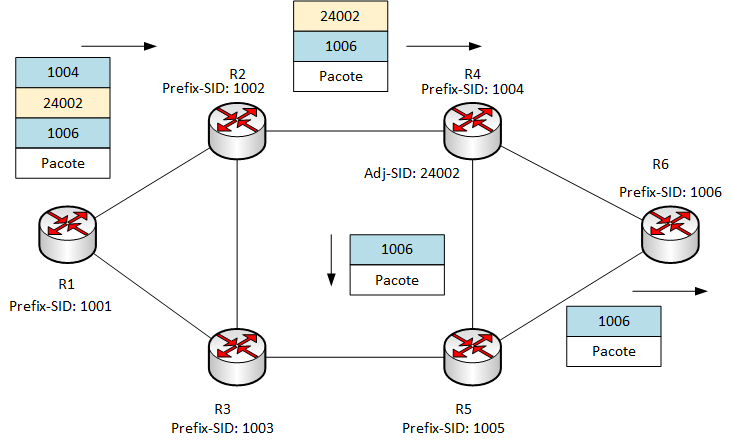
\includegraphics[width=.5\textwidth]{Segment Routing.png}
\caption{Protocolo Segment Routing - baseado em \cite{kushwaha2020survey}}
\label{fig:segmentrouting}
\end{figure}

O funcionamento do \textit{Segment Routing} é ilustrado na (Figura~\ref{fig:segmentrouting}). o nó de entrada R1 insere o pacote na rede incluindo 3 \textit{labels} \{1004, 24002 e 1006\}. O primeiro é um Prefix-SID, ou seja, é o ID do nó por onde o pacote deve passar, a rede escolhe o caminho mais adequado usando os protocolos tradicionais para ir do nó R1 até o nó R4. O label 24002 é um Adj-SID, que é o ID de uma adjacência, então o pacote é enviado pela porta que chega ao nó R5. Por fim, o Prefix-SID 1006 indica que o pacote deve ir para o nó R6. A cada troca de segmento um \textit{label} é removido do pacote e o roteador faz o \textit{repacking}, no último nó todo o encapsulamento é removido e o pacote sai do domínio \textit{Segment Routing}.

O PolKA é do tipo \textit{Strict Source Routing}, pois ele consegue explicitar todos os nós por onde o pacote deve passar, devido à forma como o protocolo foi construído. A criação do protocolo foi feita por pesquisadores do Instituto Federal de Educação do Espírito Santo (IFES), da Universidade Federal do Espírito Santo (UFES) e da Universidade de Bristol. A rota é calculada pelo controlador usando o \textit{Chinese Remainder Theorem} (CRT) e é gerado um routeID para cada rota que vai encapsular o pacote no nó de entrada. Em cada nó é realizada uma operação matemática entre o routeID da rota e o nóID, usando o resto da divisão que é calculado usando o cálculo de CRC por \textit{hardware}. O resultado é o portID que identifica por qual porta o pacote deve ser encaminhado \cite{dominicini2021deploying}.

\begin{figure}[ht]
\centering
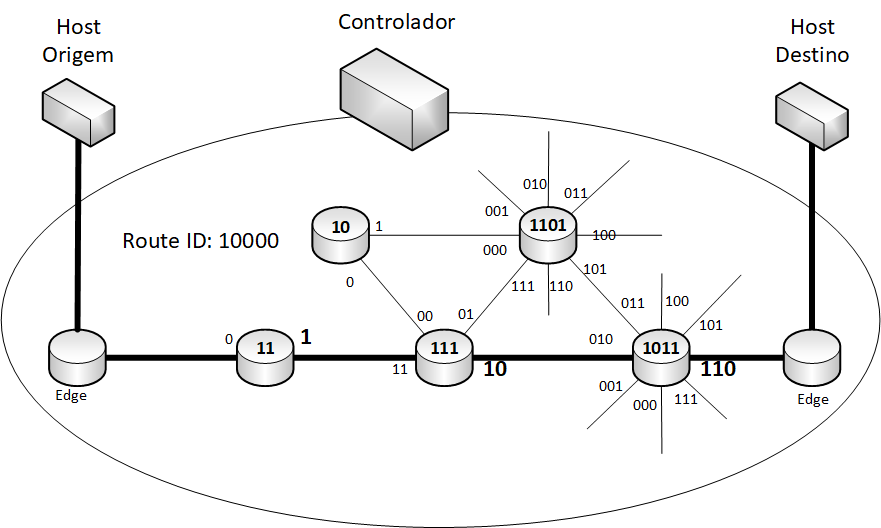
\includegraphics[width=.5\textwidth]{PolKA.png}
\caption{Protocolo PolKA - baseado em \cite{dominicini2021deploying}}
\label{fig:polka}
\end{figure}

O funcionamento do protocolo nos nós pode ser exemplificado pela Figura~\ref{fig:polka}, todos os números estão na base 2. Vemos a ilustração de uma rota que foi calculada usando o CRT pelo controlador, o RouteID 10000 faz o caminho indicado pelas linhas mais escuras. Isso ocorre porque nos nós é calculado o resto da divisão inteira de 10000 pelos IDs dos nós resultando no número da porta por onde o pacote deve ser enviado. A partir da origem o pacote entre pelo nó de borda e recebe o cabeçalho PolKA contendo o routeID 10000. No nó 11 o resto da divisão resulta em 1, o pacote segue pela porta 1 para o nó 111. O resto da divisão agora é 10 e o pacote segue para o nó 1011, onde o cálculo resulta em 110 e o pacote chega ao nó de borda, onde o pacote é desencapsulado e entregue ao destino.

A decisão de como distribuir a carga, criar novas rotas e evitar enlaces congestionados fica por conta do controlador pelo uso de algum algoritmo eficiente de engenharia de tráfego e não faz parte deste estudo.

\subsection{Requisitos de rede para aplicações de Ciência de Dados Intensiva}

O Departamento de Energia dos Estados Unidos gerencia uma das redes que integra pesquisas que geram um volume da dados muito alto, em seu relatório \textit{High Energy Physics Network Requirements Review Final Report} \cite{zurawski2021} apresenta detalhes sobre os requisitos das aplicações de Ciência de Dados Intensivas, um quadro comparativo pode ser observado na Tabela~\ref{tab:Tabela2} contendo quatro pesquisas, a capacidade de seus enlaces e o volume de dados trafegados.

\begin{table}[ht]
\centering
\caption{Centros de Pesquisa, capacidade dos enlaces de dados e volume de tráfeco}
\label{tab:Tabela2}
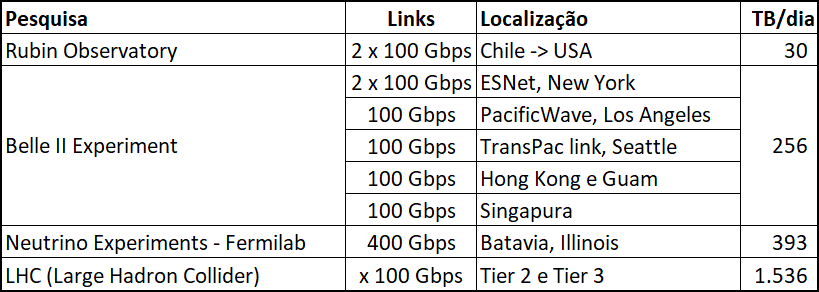
\includegraphics[width=.7\textwidth]{volumes.png}
\end{table}

O Rubin Observatory localizado no deserto do Atacama no Chile envia dados todas as noites para os laboratórios no Estados Unidos. Possui dois enlaces para redundância, durante a operação normal utiliza um dos enlaces para envio das imagens, com aproximadamente 30 TB cada, enquanto o outro enlace é usado para dados de comando e controle.

Belle II Experimento é a terceira geração de experimentos com mésons B, gera entre 7 e 8 PB de dados por mês e já atingiu picos de 12 PB. O projeto está em expansão a vai contar com pesquisadores por todo o mundo, possui dois enlaces de 100 Gbps com a ESNet e enlaces de 100 Gbps com outras redes intercontinentais.

O Neutrino Experiments está localizado dentro do Fermilab, são feitas pesquisas sobre os Neutrinos que são partículas subatômicas oriundas do sol e de supernovas, para que os dados coletados no acelerador de partícula, são usados circuitos de 100 Gbos e de 400 Gbps. Os vários experimentos executados geram um volume de dados que, quando somados, totalizam aproximadamente 393 TB por dia.

O LHC (Grande Colisor de Hádrons, do inglês \textit{Large Hadron Collider}) possui quatro colisores, o maiore deles é o ATLAS e seus dados fluem por uma rede dividida em três camadas. O colisor gera um volume muito grande em um curto espaço de tempo que precisa ser aliviado para que novos experimentos sejam executados, os equipamentos das camadas mais internas da rede estão localizados mais próximos e os enlaces são de maior capacidade. Os enlaces da camada 3 são de até 100 Gbps, com previsão de expansão para enlaces na ordem de Tbps a partir de 2028. Estes enlaces interligam a rede do ATLAS à outras redes de pesquisa geograficamente distantes. Entre 1 e 2 TB de dados são migrados diariamente para os centros de pesquisa interligados.

Para disponibilizar seus dados o Rubin Observatory organiza um catálogo usando um gerenciador de banco de dados relacional paralelo chamado Qserv, para transferir grandes arquivos é utilizado o protocolo XROOTD. O Neutrino Experiments também utiliza o protocolo XROOTD para distribuir os dados adquiridos pelos equipamentos.

Para transferência de arquivos, o ATLAS no LHC e o Belle II Experiment utilizam a ferramenta Rucio para organizar, gerenciar e acessar os arquivos. Para realizar a transferência de arquivos o Rucio utiliza o FTS (do inglês \textit{File Transfer Service}). O FTS é o serviço responsável pela distribuição de dados do LHC, utiliza a biblioteca GFAL2 (do inglês \textit{Grid File Access Library}) para realizar o trabalho pois foi criada para cópia de arquivos em ambientes de \textit{grids} e \textit{clouds}. O suporte aos métodos de cópia depende dos plugins instalados, estão disponíveis: sistema de arquivos local, SRM (que usa internamente GridFTP, FTP e HTTP), GSIFTP (ou GridFTP), HTTP, HTTPS, WebDav, XROOTD, DCAP, GSIDCAP e KDCAP.

Todos os protocolos de transferência de arquivos citados funcionam sob o protocolo TCP. O GridFTP possui uma particularidade que é a realização de transferência utilizando várias conexões simultâneas, gerando assim diversos fluxos de dados.

\subsection{SDN}

Equipamentos de rede tradicionais possuem dois planos internos para execução de rotinas predefinidas pelo fabricante. Um plano de controle permite a interação com o usuário que vai utilizar os recursos para configurar o equipamento determinando assim o seu comportamento na rede e um plano de dados que trata de fazendo o encaminhamento de pacotes entre as várias interfaces de rede. Novos equipamentos tem sido construídos tendo como base as SDNs (Redes Definidas por Software, do inglês \textit{Software Defined Networks}), neste modelo o equipamento implementa um plano de dados programável enquanto o plano de controle é executado em equipamentos externos que fazem o gerenciamento da rede. A estratégia das SDNs é superior às redes tradicionais pois os planos de controle possuem uma visão global da rede e podem tomar ações redirecionando fluxos nos planos de dados gerenciados.

\subsection{RARE/freeRtr}

O RARE/freeRtr é uma plataforma de plano de controle escrita em Java e C que utiliza sockets UDP, possui suporte à maioria dos protocolos tradicionais e aos protocolos \textit{Segment Routing} e PolKA utilizados nesta pesquisa. O RARE/freeRtr pode ser usado para emular redes ou servir como plano de controle para dispositivos de hardware especializados. Essa flexibilidade permitiu a criação da configuração de topologias similares às físicas para testar os recursos antes de partir para a implementação.

A implementação do PolKA no RARE/freeRtr permite a criação de túneis de forma simplificada e integrada à interface de configuração.

\subsection{P4}

Planos de dados podem ser programados por meio de linguagens construídas especificamente para este fim. P4 é uma das linguagens mais usadas nos equipamentos comerciais e possui uma arquitetura otimizada para fazer o encaminhamento de dados em uma rede. Apesar de existirem implementações em P4 para os protocolos tradicionais a sua grande vantagem é a possibilidade de testar novos protocolos que ainda nem foram implementados pelo fabricante ou que estão em desenvolvimento.

\subsection{bmv2}

Como plano de dados utilizamos um software emulador de \textit{switch} P4 chamado bmv2 (do inglês \textit{behavioral model version 2}). Versões em P4 dos protocolos PolKA e \textit{Segment Routing} foram implantadas no emulador para que fosse possível executar os testes no ambiente emulado.

\subsection{Global P4 Lab}

O GLobal P4 Lab é um \textit{testbed} que possui vários \textit{switches} programáveis P4 na Europa, Estados Unidos e Brasil. O \textit{testbed} foi utilizado para executar os experimentos em dispositivos físicos, replicando os testes realizados nos ambientes virtuais. A disposição geográfica da rede pode ser vista na Figura~\ref{fig:p4lab}.

\begin{figure}[ht]
\centering
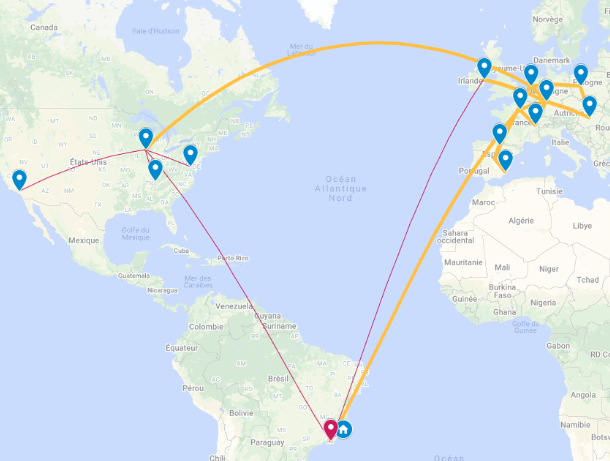
\includegraphics[width=.5\textwidth]{p4lab.png}
\caption{Rede Global P4 Lab}
\label{fig:p4lab}
\end{figure}

\subsection{iperf}

Para geração de fluxo de dados usamos o iperf \cite{esnet}, a ferramenta permite funcionar como cliente ou servidor e serve para injetar tráfego na rede e medir taxa de transferência/\textit{bitrate}, perda e outros parâmetros.

\subsection{DPDK}

O DPDK (Data Plane Development Kit) é um conjunto de bibliotecas usadas para acelerar as cargas de trabalho no processamento de pacotes, ele é útil para que na geração de diversos fluxos a máquina consiga ocupar todo o enlace disponível, isso não é possível utilizando o driver de rede tradicional.


O ambiente de testes selecionado para instalação das ferramentas foi o Linux Ubuntu 22.04 LTS.

\section{Avaliação do Artigo}

Os experimentos foram planejados com o objetivo de avaliar como os dois protocolos se comportam em uma rede de alto desempenho ao trafegar um grande volume de dados gerado por meio de diversos fluxos em paralelo.

\subsection{Método}

Os experimentos foram executados em ambiente emulado e, após a coleta dos resultados, foram executados em ambiente real, nos \textit{testbeds} internacionais.
No ambiente virual utilizamos o RARE/freeRtr como plano de controle, bmv2 como plano de dados com suporte ao P4 e iperf para gerar os fluxos de dados.
Nos \testit{testbeds} físicos utilizamos o RARE/freeRtr com plano de controle, \textit{switches} Intel Tofino com suporte ao P4 e iperf na geração dos fluxos de dados.

\section{Os experimentos}

O objetivo dos experimentos é verificar se os protocolos \textit{Segment Routing} e PolKA conseguem atingir os requisitos das aplicações de Ciências de Dados Intensivas.

Como as aplicações enviam um volume muito grande de dados e eles precisam ser recebidos no menor espaço de tempo possível, é importante ocupar toda a largura de banda disponível. Uma vez que as redes científicas estão utilizando enlaces de, pelo menos, 100Gbps para conexão aos centros de pesquisa, precisamos atingir uma taxa de transferência que ocupe o enlace disponível chegando a picos próximos da sua capacidade nominal.

Outra característica das aplicações de ciências de dados intensivas é o uso de vários fluxos simultâneos. Dessa forma, utilizamos fluxos agregados para chegar ao limite de uso da rede. O uso do DPDK e parametrização do Kernel Linux foram necessários para atingir esse objetivo.

\subsection{Experimento 1 - Configuração de túneis e Agregação de fluxos para vazão de 100Gbps}

Para verificar se as implementações dos protocolos conseguem atingir a vazão de \textit{line rate} de 100Gbps dos equipamentos com o uso da agregação de múltiplos fluxos.

Utilizamos a topologia mostrada na Figura~\ref{fig:topologia2}.

\begin{figure}[ht]
\centering
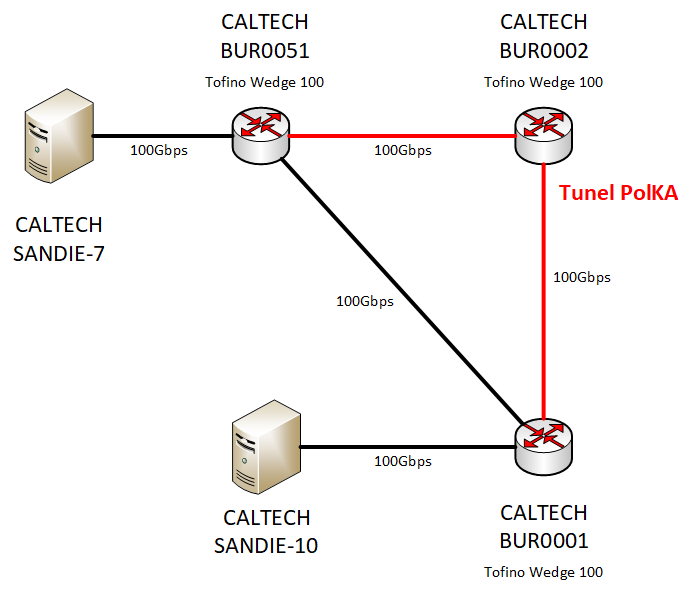
\includegraphics[width=.5\textwidth]{Topologias-polka 2.png}
\caption{Topologia do teste de agregação de enlace}
\label{fig:topologia2}
\end{figure}

O teste realizado dentro da Caltech utilizou três \textit{switches} Tofino da Intel em uma rede local. Foi criado um tunel PolKA criando o caminho BUR0051 $\rightarrow$ BUR0002 $\rightarrow$ BUR0001.

Para criar um tunel PolKA no RARE/freeRtr usamos a interface e especificamos os parâmetros conforme ilustrado na Figura~\ref{fig:tunel1}. O parâmetro domain-name define o caminho por onde o pacote deve trafegar. Ao configurar o túnel será definido o routeID que será inserido no cabeçalho, este valor pode ser visto com o comando "show polka routid <nome-do-túnel>" conforme apresentado na Figura~\ref{fig:tunel2}. O routeID será usado pelos nós da rede, o resultado da operação de resto da divisão entre routeID e o nodeID vai resultar na porta por onde o pacote deve ser encaminhado.

\begin{figure}[ht]
\centering
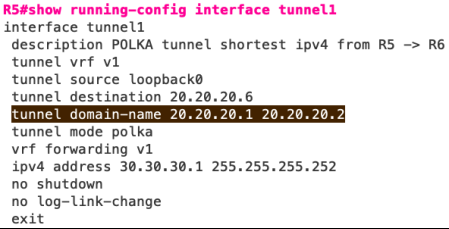
\includegraphics[width=.5\textwidth]{tunel1.png}
\caption{Configuração do túnel PolKA \cite{borges2022lifecycle}}
\label{fig:tunel1}
\end{figure}

\begin{figure}[ht]
\centering
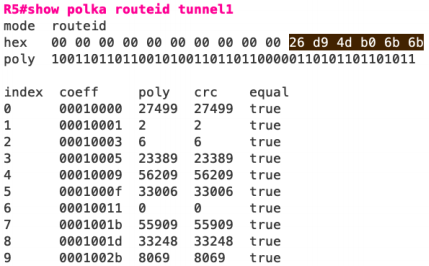
\includegraphics[width=.5\textwidth]{tunel2.png}
\caption{Visualizando o routeID do túnel PolKA \cite{borges2022lifecycle}}
\label{fig:tunel2}
\end{figure}

No equipamento Sandie7 foram criados quatro fluxos de dados com destino ao equipamento Sandie10 usando o software iperf. Estes fluxos foram acionados um sequência enquanto usamos o software bwm-ng para monitorar o estado da interface de rede da máquina de destino.

Pelo acionamento sequencial dos fluxos conseguimos observar que a ocupação do enlace também foi gradual. Ao acionar o último fluxo, conseguimos atingir quase a ocupação total de 100 Gbps, a diferença foi bem pequena e está relacionada com a sobrecarga necessária para o controle da rede e sistema operacional da máquina.

Para que as máquinas de origem e destino atingissem taxas tão altas foi necessário utilizar o DPDK, além de fazer alguns ajustes nos parâmetros do kernel Linux a fim de evitar que interrupções do sistema operacional causem interferências.

Na Figura~\ref{fig:agregacao} pode ser observado que ao subir o último dos quatro fluxos o enlace chegou próximo da sua capacidade nominal de 100 Gpbs. A ocupação máxima do enlace é um dos requisitos que buscamos atender com os experimentos.

\begin{figure}[ht]
\centering
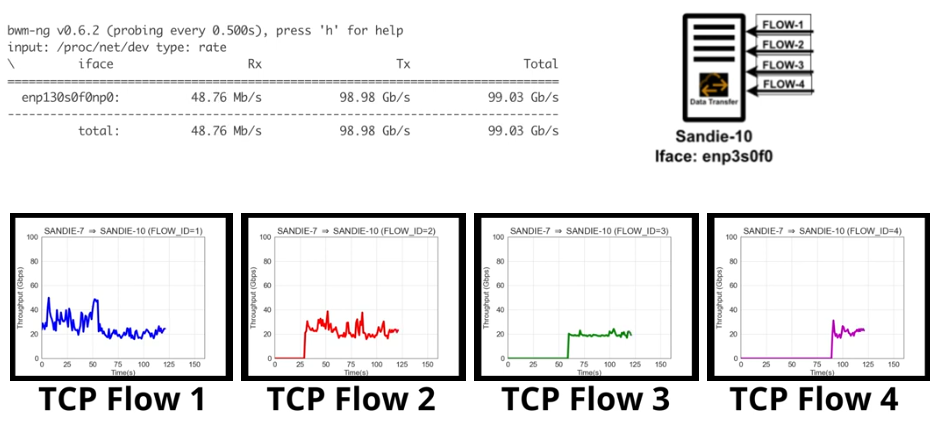
\includegraphics[width=.5\textwidth]{AgregacaoLink.png}
\caption{Agregação de fluxos - Ocupação do enlace}
\label{fig:agregacao}
\end{figure}

\subsection{Experimento 2 - Mudança de instância de serviço por meio de migração de túnel}

A tolerância à falhas também é um recurso imprescindível que deve estar presente nas redes científicas, para avaliar esse comportamento foi utilizado a topologia de rede da Figura~\ref{fig:topologia1}.

\begin{figure}[ht]
\centering
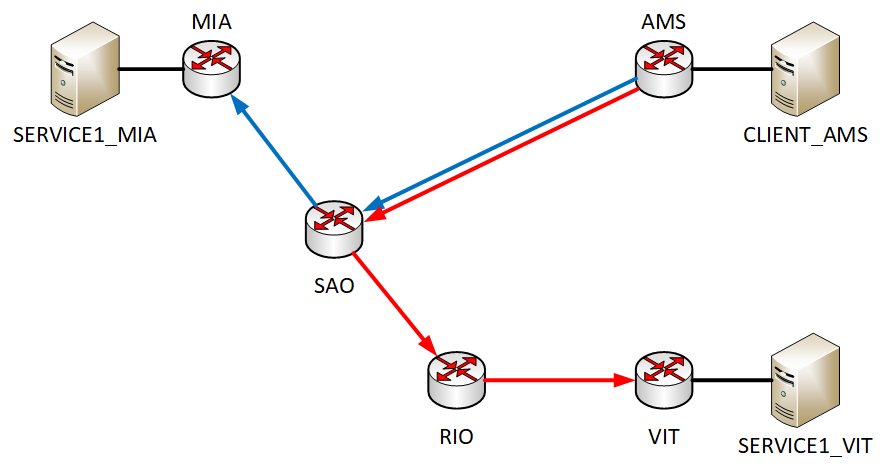
\includegraphics[width=.5\textwidth]{Topologias-polka 1.png}
\caption{Topologia do teste de migração de enlace}
\label{fig:topologia1}
\end{figure}

Neste experimento temos um cliente localizado em Amsterdã (AMS) que utiliza um serviço espelhado em dois servidores, um  localizado em Miami (MIA) e outro em Vitória (VIT).

O roteador de borda localizado em AMS insere no pacote a rota desejada. Iniciamos com o servidor em MIA que possui um enlace com maior latência. Depois, com o cliente em funcionamento trocamos no roteador de borda a rota para que os pacotes passem a ser enviados para São Paulo (SAO), Rio de Janeiro (RIO) e VIT, que entrega ao servidor espelho.

Foi utilizado o software iperf para gerar o fluxo de dados entre o cliente e o servidor, na Figura~\ref{fig:migracao} é possível observar que ao trocar a a rota temos imediatamente uma diminuição do RTT (do inglês \textit{Round Trip Time}) de 256 ms para 171 ms, indicando uma diminuição no tempo de resposta do protocolo ICMP. Como os dois servidores usam o mesmo endereço IP, o cliente não percebe a troca de servidor durante o acesso ao serviço espelhado.

A migração de túnel atende ao requisito de uso eficiente da rede ao permitir que o controlador redirecione o tráfego por rotas menos utilizadas. Serviços replicados também podem ser migrados de forma transparente para as aplicações.

\begin{figure}[ht]
\centering
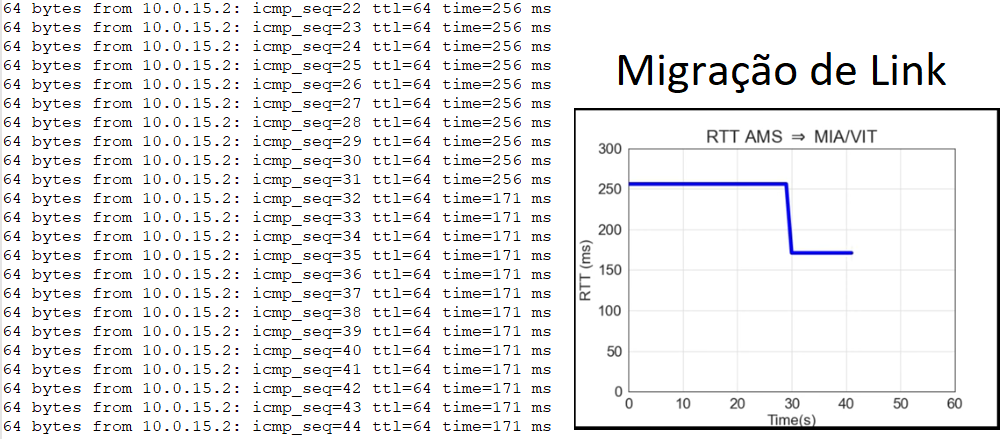
\includegraphics[width=.5\textwidth]{MigracaoLink.png}
\caption{Migração de enlace - troca de rota}
\label{fig:migracao}
\end{figure}


\subsection{Experimento 3 - Balanceamento de carga e recuperação a falhas}

Utilizamos a topologia mostrada na Figura~\ref{fig:topologia3} para realizar o teste de balanceamento de carga e \textit{failover}. O experimento é similar ao primeiro teste mas, nesse caso, a origem e o destino são os mesmos. Em caso de falha no caminho em uso, podemos mudar a rota para o caminho alternativo e a aplicação cliente continuará se comunicando com o servidor sem interrupções.

\begin{figure}[ht]
\centering
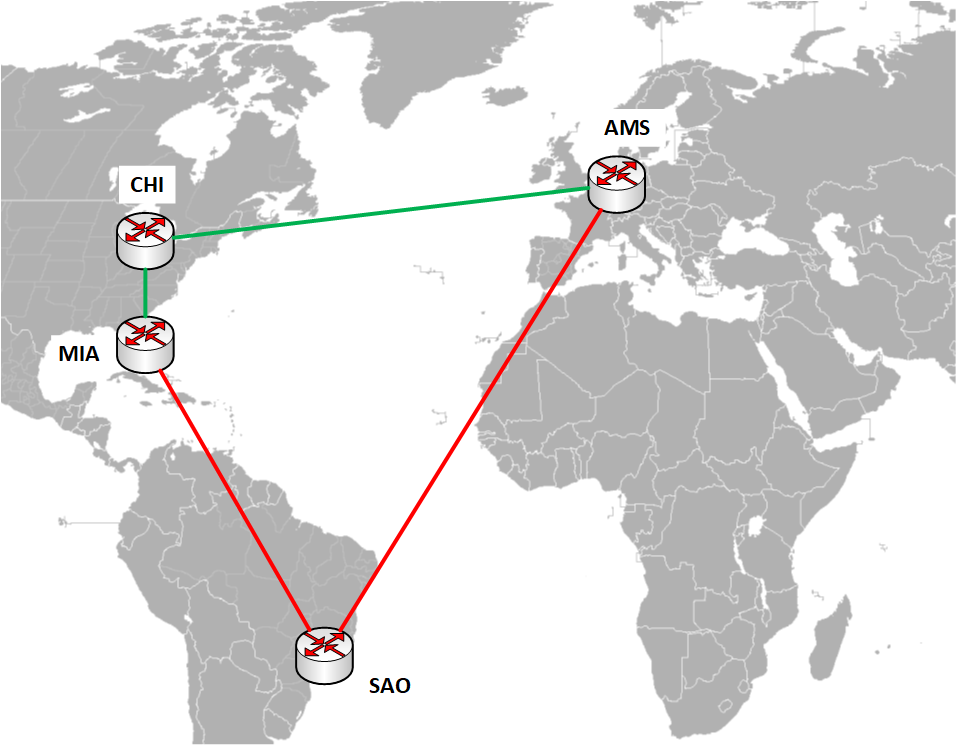
\includegraphics[width=.5\textwidth]{Topologias-polka 3.png}
\caption{Topologia do teste de balanço de carga/failover}
\label{fig:topologia3}
\end{figure}

O cliente foi conectado ao \textit{switch} de borda em Miami (MIA) e o \textit{switch} de borda em Amsterdã (AMS) está conectado ao servidor.

Criamos dois túneis PolKA, um passando por Chicago (CHI) e outro por São Paulo (SAO), utilizamos dois fluxos criados com o iperf no cliente e regras no roteador de borda em MIA para que cada fluxo passe por uma rota.

Durante a transmissão de dados, modificamos uma das regras para que os pacotes passem por outro túnel. O \textit{switch} de borda passou a encaminhar todos os pacotes por SAO mostrando como o fluxo pode ser direcionado em tempo real para uma nova rota no caso de uma falha na rota original.

Usando a mesma técnica é possível segmentar o fluxo de dados na rede usando rotas alternativas que estejam subutilizadas, dar prioridade a fluxos com maior importância, reservar circuitos para experimentos específicos e outras funções características da engenharia de tráfego. Os requisitos de recuperação a falhas e uso eficiente da rede é atingido com o uso da mudança dos túneis no roteador de borda.

\bibliographystyle{sbc}
\bibliography{sbc-template}

\end{document}
